% !TeX document-id = {5c581797-4493-4c49-83e2-2f6935aa95ee}
% !TeX TXS-program:compile = txs:///xelatex/[--shell-escape]
% !TeX spellcheck = en_US

%%%%%%%%%%%%%%%%%%%%%%%%%%%%%%%%%%%%%%%%%%%%%%%%%%%%%
%%%%%%%%%%%%%%%%%%%%%%%%%%%%%%%%%%%%%%%%%%%%%%%%%%%%%

%%%%%%%%%%%%%%%%%%% BEGIN OF HEAD %%%%%%%%%%%%%%%%%%%

%\documentclass[10pt,english,aspectratio=169]{beamer} % With animations
\documentclass[10pt,english,handout,aspectratio=169]{beamer} % Without animations (for printing)
\setbeamertemplate{theorems}[numbered] % To number theorems, lemmas, definitions...

\usetheme[numbering=fraction,progressbar=frametitle,block=fill,subsectionpage=progressbar]{metropolis}

% For the code, so it looks like real code
\usepackage{fontspec}
\setmonofont{Iosevka Term}

\newfontfamily\DejaSans{DejaVu Sans} %Emojis

% https://tex.stackexchange.com/questions/60360/how-to-use-fraktur-gothic-fonts-in-text-mode
\usepackage{yfonts} %Gothic Font e.g., \textgoth{}
\usepackage{mathrsfs} %Used for super caligraphic font \mathscr{}

% Footnote size
\setbeamerfont{footnote}{size=\tiny} 

% Animation transparent
\setbeamercovered{transparent}

% To import Inkscape figures
\usepackage{import}
\usepackage{pdfpages}
\usepackage{transparent}
\usepackage{xcolor}

% To create an appendix
\usepackage{appendixnumberbeamer}

% Metropolis dependences
\usepackage{etoolbox}
\usepackage{ifxetex}
\usepackage{pgfopts}
\usepackage{calc}
\usepackage{ifluatex}

% Tikz Library
% https://www.iacr.org/authors/tikz/
\usepackage{tikz}
\usetikzlibrary{shapes.callouts,calc, arrows, positioning, matrix, intersections, decorations.markings}
\tikzset{point/.style={draw,fill,circle,inner sep=1pt}}
\tikzset{vertex/.style = {shape=circle,draw,minimum size=1.5em}}
\tikzset{line/.style = {-}}
\tikzset{arrow/.style = {->}}

\newcommand{\plotcurve}[4][thick, every plot/.style={smooth}]{
  % plot curve y^2 = x^3 + a x + b in range [-#4,#4]^2
  % parameter 1 (optional): style options for curve (color, etc)
  % parameter 2: curve parameter a
  % parameter 3: curve parameter b
  % parameter 4: range to print
  % \draw[gray] (-3,-3) rectangle (3,3);
  \draw[->,>=latex,gray] (-#4,0) -- (#4,0);
  \draw[->,>=latex,gray] (0,-#4) -- (0,#4);
  \draw[name path=curve, #1] plot[id=curve#2#3, raw gnuplot] function {
    f(x,y) = y**2 - x**3 - #2*x - #3;
    set xrange [-#4:#4];
    set yrange [-#4:#4];
    set view 0,0;
    set isosample 50,50;
    set contour base;
    set cntrparam levels incre 0,0.1,0;
    unset surface;
    splot f(x,y);
  };
}

% For an explanation of the tangent coordinate system, check http://tex.stackexchange.com/a/25940 
\tikzset{
  tangent/.style={
    decoration={markings, mark=at position #1 with {
      \coordinate (tangent point-\pgfkeysvalueof{/pgf/decoration/mark info/sequence number}) at (0pt,0pt);
      \coordinate (tangent unit vector-\pgfkeysvalueof{/pgf/decoration/mark info/sequence number}) at (1,0pt);
      \coordinate (tangent orthogonal unit vector-\pgfkeysvalueof{/pgf/decoration/mark info/sequence number}) at (0pt,1);
    }},
    postaction=decorate
  },
  use tangent/.style={
    shift=(tangent point-#1),
    x=(tangent unit vector-#1),
    y=(tangent orthogonal unit vector-#1)
  },
  use tangent/.default=1
}

% Alternative to tikz
\usepackage{pgfplots}
\pgfplotsset{compat=newest}

% This package controls how hyperlinks are displayed
% https://es.overleaf.com/learn/latex/Hyperlinks
\usepackage{hyperref}
\hypersetup{colorlinks=true,linkcolor={red!80!black},urlcolor={blue!80!black}}

% A better version of the proof environtment for beame
% The optional parameter is though to be "of Lemma \ref{ref-to-the-lemma}" or "of Theorem \ref{ref-to-the-theorem}"
\renewenvironment{proof}[1][\unskip]{\textbf{Proof #1:} \vspace{1mm} \hrule \vspace{1mm}}{\hfill$\qed$ \vspace{1mm} \hrule \vspace{1mm}}

% Benaloh Brackets
\usepackage{stmaryrd}

% Quotes: \enquote
\usepackage{csquotes}

% Cancel out math
\usepackage{cancel}

%This ensures spaces when using ensuremath and no $$ are used to introduce math
\usepackage{xspace}

% Working directory
\newcommand{\definedir}[2]{\newcommand{#1}{#2}}
\definedir{\zkevmdir}{..}

% Path relative to the main .tex file 
\graphicspath{{\zkevmdir/architecture/figures/}}

%\newcommand{\incfig}[2][1]{%
%	\def\svgwidth{#1\columnwidth}
%	\import{\dir/figures/}{#2.pdf_tex}
%}

% Table of contents configuration
\AtBeginSection[]
{
\begin{frame}
	\setcounter{tocdepth}{1} %show only up to section
	\frametitle{Table of Contents}
  \hypersetup{linkcolor=.}
	\tableofcontents[currentsection,
		sectionstyle=show/shaded] %currentSection/anotherSections
\end{frame}
}

\AtBeginSubsection[]
{
\begin{frame}
	\setcounter{tocdepth}{2} %show only up to subsection
	\frametitle{Table of Contents}
  \hypersetup{linkcolor=.}
	\tableofcontents[currentsection,
        currentsubsection,
		sectionstyle=show/shaded, %currentSection/anotherSections
        subsectionstyle=show/shaded/hide]
		%currentSubSeciont - currentSection/
		%anotherSubSeciont - currentSection/
		%SubSeciont - anotherSection
\end{frame}
}

%%%%%%%%%%%%%%%%%%% END OF HEAD %%%%%%%%%%%%%%%%%%%%

%%%%%%%%%%%%%%%%%%%%%%%%%%%%%%%%%%%%%%%%%%%%%%%%%%%%
%%%%%%%%%%%%%%%%%%%%%%%%%%%%%%%%%%%%%%%%%%%%%%%%%%%%

%%%%%%%%%%%%%%% BEGIN OF LSTLISTINGS %%%%%%%%%%%%%%%

\usepackage{showexpl}% already includes listings package
% The listings package defines an internal command for replacements within filenames. 
% One of these replacements replaces - with \textendash. 
% You can redefine this command to make the hyphens actual hyphens:
\makeatletter
\def\lst@filenamerpl{_\textunderscore $\textdollar}
\makeatother
\lstset{
	frame=shadowbox, 
	basicstyle=\footnotesize\ttfamily, 
	showstringspaces=false,
	rulesepcolor=\color{black}, 
	upquote=true
}
% \lstset{language=bash, frame=shadowbox, basicstyle=\footnotesize, showstringspaces=false,
% rulesepcolor=\color{black}, upquote=true, }
\lstdefinestyle{scriptStyle}{
	basicstyle=\footnotesize,% control font of code
	preset=\footnotesize,% adjust font size of output
	numbers=left, numberstyle=\tiny, stepnumber=1, numbersep=5pt,
	frame=tlbr,
	pos=r,% want output on rightbackgroundcolor=\color{yellow!30},
	width=0.50\linewidth,
}

\lstdefinestyle{terms}{
	basicstyle=\scriptsize\ttfamily,% control font of code
	preset=\footnotesize,% adjust font size of output
}

\lstdefinestyle{termt}{
	basicstyle=\tiny\ttfamily,% control font of code
	preset=\footnotesize,% adjust font size of output
}

\lstdefinestyle{verb}{
	basicstyle=\footnotesize,% control font of code
	preset=\footnotesize,% adjust font size of output
	frame=tlbr,
	pos=r,% want output on right
	%     backgroundcolor=\color{yellow!30},
	width=0.50\linewidth,
}

\lstdefinestyle{verbs}{
	basicstyle=\scriptsize,% control font of code
	preset=\scriptsize,% adjust font size of output
	frame=tlbr,
	pos=r,% want output on right
	%     backgroundcolor=\color{yellow!30},
	width=0.50\linewidth,
}

\lstdefinestyle{verbt}{
	basicstyle=\tiny\ttfamily,% control font of code
	preset=\tiny\ttfamily,% adjust font size of output
	frame=tlbr,
	pos=r,% want output on right
	%     backgroundcolor=\color{yellow!30},
	width=0.50\linewidth,
}

%%%%%%%%%%%%%%%%% END OF LSTLISTINGS %%%%%%%%%%%%%%%%

%%%%%%%%%%%%%%%%%%%%%%%%%%%%%%%%%%%%%%%%%%%%%%%%%%%%%
%%%%%%%%%%%%%%%%%%%%%%%%%%%%%%%%%%%%%%%%%%%%%%%%%%%%%

%%%%%% BEGIN OF CODE HIGHLIGHTING ENVIRONMENTS %%%%%%

%   sudo apt install texlive-latex-extra 
%   sudo apt install python-pip
%   pip install pygments
%   pip install pygments-lexer-babylon  #contains JSX
%   pip install pygments-lexer-solidity 
%   pip install pygments pygments-lexer-babylon pygments-lexer-solidity



\usepackage{tcolorbox}
\tcbuselibrary{minted,skins,listings}
\definecolor{mybg}{rgb}{0.96,0.96,0.98}

\newtcblisting{term}{
	listing engine=minted,
	colback=black,
	colframe=black!0,
	coltext=white,
	listing only,
	minted style=tango,
	minted language=text,
	minted options={linenos=false,texcl=true},
	left=0mm, top=0mm, bottom=0mm, right=0mm,
	boxrule=0mm
}

\newtcblisting{js}{
	listing engine=minted,
	colback=mybg,
	colframe=black!30,
	listing only,
	minted style=tango,
	minted language=js,
	minted options={linenos=false,texcl=true},
	left=0.2mm,
	top=0cm,
	bottom=0cm,
	boxrule=0.1mm
}

\newtcblisting{ts}{
	listing engine=minted,
	colback=mybg,
	colframe=black!30,
	listing only,
	minted style=tango,
	minted language=ts,
	minted options={linenos=false,texcl=true},
	left=0.2mm,
	top=0cm,
	bottom=0cm,
	boxrule=0.1mm
}

\newtcblisting{solidity}{
	listing engine=minted,
	colback=mybg,
	colframe=black!70,
	listing only,
	minted style=tango,
	minted language=solidity,
	minted options={linenos=false,texcl=true,fontsize=\tiny},
	left=0.2mm,
	top=0cm,
	bottom=0cm,
	boxrule=0.1mm
}

\newtcblisting{sql}{
	listing engine=minted,
	colback=mybg,
	listing only,
	minted style=tango,
	minted language=sql,
	minted options={linenos=false,texcl=true},
	left=0.2mm,
	top=0cm,
	bottom=0cm,
	colframe=black!30,
	boxrule=0.1mm
}

%%%%%%% END OF CODE HIGHLIGHTING ENVIRONMENTS %%%%%%%

%%%%%%%%%%%%%%%%%%%%%%%%%%%%%%%%%%%%%%%%%%%%%%%%%%%%%%%
%%%%%%%%%%%%%%%%%%%%%%%%%%%%%%%%%%%%%%%%%%%%%%%%%%%%%%%

%%%%%%%%%%%%%%%%%%% BEGIN OF MACROS %%%%%%%%%%%%%%%%%%%

% Cryptocode: https://github.com/arnomi/cryptocode
% You have to update the package manually by downloading the latest ".sty" in the link above and then:
% sudo mv ~/cryptocode.sty usr/share/texlive/texmf-dist/tex/latex/cryptocode
\usepackage[
lambda,
operators,
landau, %este es el de bigO
probability,
%sets,
logic, %para or,and...	
asymptotics,
keys
]{cryptocode}

% My own procedure blocks to show protocols
\createprocedureblock{mypb}{center, boxed}{}{}{linenumbering}
\createprocedureblock{mypbnonum}{center, boxed}{}{}{}

% Numbering style
\renewcommand{\pclnstyle}[1]{\text{#1}}
\renewcommand{\pclnseparator}{.}

%%%%%%%%%%%%%%%%%%%%%%%%%%%%%%%%%%%%%%%%%%%%%%%%%%%%%%%%

% Hyphen inside mathmode
\mathchardef\mhyphen="2D

% Bold Math
\renewcommand{\vec}[1]{\ensuremath{\boldsymbol{#1}}\xspace}
\newcommand{\vel}[3]{\ensuremath{\vec{#1_{#2}}(#3)}\xspace}

% Mathbb
\renewcommand{\AA}{\ensuremath{\mathbb{A}}\xspace}
\newcommand{\CC}{\ensuremath{\mathbb{C}}\xspace}
\newcommand{\FF}{\ensuremath{\mathbb{F}}\xspace}
\newcommand{\GG}{\ensuremath{\mathbb{G}}\xspace}
\newcommand{\KK}{\ensuremath{\mathbb{K}}\xspace}
\newcommand{\NN}{\ensuremath{\mathbb{N}}\xspace}
\newcommand{\PP}{\ensuremath{\mathbb{P}}\xspace}
\newcommand{\QQ}{\ensuremath{\mathbb{Q}}\xspace}
\newcommand{\RR}{\ensuremath{\mathbb{R}}\xspace}
\newcommand{\ZZ}{\ensuremath{\mathbb{Z}}\xspace}

% Mathcal
\newcommand{\B}{\ensuremath{\mathcal{B}}\xspace}
\renewcommand{\C}{\ensuremath{\mathcal{C}}\xspace}
\newcommand{\E}{\ensuremath{\mathcal{E}}\xspace}
\renewcommand{\H}{\ensuremath{\mathcal{H}}\xspace}
\newcommand{\I}{\ensuremath{\mathcal{I}}\xspace}
\newcommand{\K}{\ensuremath{\mathcal{K}}\xspace}
\newcommand{\M}{\ensuremath{\mathcal{M}}\xspace}
\renewcommand{\O}{\ensuremath{\mathcal{O}}\xspace}
\renewcommand{\P}{\ensuremath{\mathcal{P}}\xspace}
\newcommand{\Q}{\ensuremath{\mathcal{Q}}\xspace}
\newcommand{\R}{\ensuremath{\mathcal{R}}\xspace}
\renewcommand{\S}{\ensuremath{\mathcal{S}}\xspace}
\newcommand{\T}{\ensuremath{\mathcal{T}}\xspace}
\newcommand{\V}{\ensuremath{\mathcal{V}}\xspace}
\newcommand{\X}{\ensuremath{\mathcal{X}}\xspace}

% Mathscr
\newcommand{\CCC}{\ensuremath{\mathscr{C}}\xspace}
\newcommand{\PPP}{\ensuremath{\mathscr{P}}\xspace}

% Mathfrak
\newcommand{\z}{\ensuremath{\mathfrak{z}}\xspace}

% Caligraphic Combiantions
\DeclareMathAlphabet{\mathpgoth}{OT1}{pgoth}{m}{n}
\newcommand{\plonk}{\ensuremath{\mathcal{P}\mathfrak{lon}\mathcal{K}}\xspace}
\newcommand{\fflonk}{\ensuremath{\mathcal{FF}\mathfrak{lon}\mathcal{K}}\xspace}
\newcommand{\plookup}{\ensuremath{\mathpgoth{plookup}}\xspace}

% Abbreviations
\newcommand{\eqstackrel}[2]{\ensuremath{\stackrel{\substack{\mathclap{#2}\\[0.5ex]\displaystyle\uparrow\\ ~}}{#1}}\xspace} %this is used to justify any symbol #1
\newcommand{\Pp}{\ensuremath{\mathcal{P}_{\mathsf{poly}}}\xspace}
\newcommand{\Vp}{\ensuremath{\mathcal{V}_{\mathsf{poly}}}\xspace}
\newcommand{\MR}{\ensuremath{\mathsf{MR}}\xspace}
\renewcommand{\deg}{\ensuremath{\mathsf{deg}}\xspace}
\newcommand{\inp}{\ensuremath{\mathsf{in}}\xspace}
\newcommand{\set}{\ensuremath{\mathsf{set}}\xspace}
\newcommand{\op}{\ensuremath{\mathsf{op}}\xspace}

% Symbols over arrows
\newcommand{\eqI}{\ensuremath{\overset{?}{=}}\xspace}
\newcommand{\leftR}{\ensuremath{\leftarrow_R}\xspace}

% Operator abreviattion
\renewcommand{\gcd}{\ensuremath{\mathsf{gcd}}\xspace}
\renewcommand{\max}{\ensuremath{\mathsf{max}}\xspace}
\renewcommand{\log}{\ensuremath{\mathsf{log}}\xspace}
\newcommand{\lcm}{\ensuremath{\mathsf{lcm}}\xspace}
\renewcommand{\mod}[1]{\ensuremath{~(\mathsf{mod}~#1)}\xspace}
\newcommand{\Mod}[1]{\ensuremath{~\mathsf{mod}~#1}\xspace}
\newcommand{\legendre}[2]{\ensuremath{\left(\frac{#1}{#2}\right)}\xspace}
\newcommand{\Bracket}[1]{\ensuremath{\left[#1\right]}\xspace}
%\newcommand{\Bracket}[1]{\ensuremath{\llbracket#1\rrbracket}\xspace} %Benaloh Bracket

%Name of a function: ensuremath and xspace does not work for them
\DeclareMathOperator{\DFT}{DFT} 
\DeclareMathOperator{\PI}{PI} 

% Make a nice emptyset
\let\oldemptyset\emptyset
\let\emptyset\varnothing

% Make a nice phi
\let\oldphi\phi
\let\phi\varphi
	
% Make a nice q.e.d. symbol
\renewcommand\qedsymbol{\ensuremath{\blacksquare}\xspace}

%%%%%%%%%%%%%%%%%%% END OF MACROS %%%%%%%%%%%%%%%%%%%

%%%%%%%%%%%%%%%%%%%%%%%%%%%%%%%%%%%%%%%%%%%%%%%%%%%%%
%%%%%%%%%%%%%%%%%%%%%%%%%%%%%%%%%%%%%%%%%%%%%%%%%%%%%

%%%%%%%%%%%%%%%%%%%%%%%%%%%%%%%%%%%%%%%%%%%%%%%%%%%%%%
%%$$$$$$$$$$$         TITLE PAGE	     %%$$$$$$$$$$$ 
%%%%%%%%%%%%%%%%%%%%%%%%%%%%%%%%%%%%%%%%%%%%%%%%%%%%%%
%%$$$$$$$$$$$             ||             %%$$$$$$$$$$$
%%$$$$$$$$$$$             ||             %%$$$$$$$$$$$
%%$$$$$$$$$$$             \/             %%$$$$$$$$$$$


% Titlepage
\title{Zero Knowledge Ethereum Virtual Machine}
%\subtitle{Subtitle}
\author{\textbf{Jordi Baylina ~~~ Héctor Masip ~~~ Jose L. Muñoz-Tapia}}
\institute{Polygon-Hermez \\ Information Security Group, Universitat Politècnica de Catalunya (UPC)}
\date{\today}
\titlegraphic{
\includegraphics[height=1.5cm]{logos/hermez} 
\hfill 
\includegraphics[height=1.5cm]{logos/upc}
}

% Change default options for the titlepage
\setbeamertemplate{date}{
	\raggedleft%
	\raggedbottom%
	\vspace*{2mm}
	%\insertdate% %Uncomment this line to add the date
	\par%
}

%Uncomment this command to add the date
%\setbeamertemplate{institute}{
%	\vspace*{-3mm}
%	\insertinstitute%
%	\par%
%}


%%$$$$$$$$$$$             /\             %%$$$$$$$$$$$
%%$$$$$$$$$$$             ||             %%$$$$$$$$$$$
%%$$$$$$$$$$$             ||             %%$$$$$$$$$$$
%%%%%%%%%%%%%%%%%%%%%%%%%%%%%%%%%%%%%%%%%%%%%%%%%%%%%%
%%$$$$$$$$$$$         TITLE PAGE	     %%$$$$$$$$$$$ 
%%%%%%%%%%%%%%%%%%%%%%%%%%%%%%%%%%%%%%%%%%%%%%%%%%%%%%

%%%%%%%%%%%%%%%%%%% SOME USEFUL LATEX %%%%%%%%%%%%%%%%%%%

% Web for icons: https://www.flaticon.com/

% Fragile is necessary for showing code
%\begin{frame}[fragile]{}
%\end{frame}

%\begin{figure}[ht]
%	\centering
%	\incfig{}
%\end{figure}

%\begin{figure}
%	\includegraphics[width=\textwidth]{}
%\end{figure}

%\[
%\begin{array}{|c|c|c|}
%\multicolumn{number of columns}{align}{text} \\ \hline
%\hline
% & & \\ \hline
% & & \\ \hline
%\end{array}
%\]

%\begin{overprint}
%	\onslide<1>\centering
%	\includegraphics[width=\textwidth]{}
%\end{overprint}	

%\begin{columns}
%\begin{column}{0.5\textwidth}
%\end{column}
%\begin{column}{0.5\textwidth}
%\end{column}
%\end{columns}

% For smaller procedure block size
%\begin{pchstack}[boxed, center]
%\pcsetargs{codesize=\scriptsize{}}
%
%\procedure{}{}
%\end{pchstack}

%For repeating a slide
%\begin{frame}[label=test]
%\againframe{test}

% To number only some lines of align
%\begin{align}
%eq1 \nonumber \\
%eq2 \label{eq:eq-2}
%\end{align}

% To color something
% https://es.overleaf.com/learn/latex/Using_colours_in_LaTeX
%{\color{red!80!black} text}

% Function definition
%\begin{align*}
%f \colon \FF_p &\to \FF_p \\
%x &\mapsto x^k.
%\end{align*}

\begin{document}
	
\maketitle
	
\begin{frame}{Table of Contents}
  \hypersetup{linkcolor=.}
	\tableofcontents
\end{frame}
	
% !TeX spellcheck = en_GB
% !TeX root = ../../build/architecture.tex

\section{Introduction}

\begin{frame}[allowframebreaks]{First Example: The Fibonacci State Machine}

\begin{columns}
\begin{column}{0.3\textwidth}
\begin{figure}
	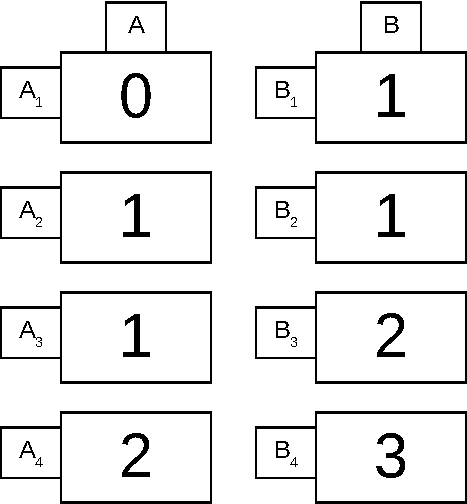
\includegraphics[width=\textwidth]{\zkevmdir/architecture/figures/fibonacci-sequence}
\end{figure}
\end{column}
%\hspace{-1.4cm}
\begin{column}{0.7\textwidth}
\begin{itemize}
\item We can build the Fibonacci state machine with two registries, $A$ and $B$.
\item In the Fibonacci sequence, we have the following relations between the states of these registries:
\begin{align*}
A_{i+1} &= B_i, \\
B_{i+1} &= A_i + B_i.
\end{align*}

\item Let's represent the states of these registries for four steps as polynomials in $\ZZ_p[x]$ evaluated 
on the group $H = \{\omega, \omega^2, \omega^3, \omega^4 = 1\}$:
\begin{align*}
A(\omega^i) &= A_i \quad \Longrightarrow \quad A = [0, 1, 1, 2] \\
B(\omega^i) &= B_i \quad \Longrightarrow \quad B = [1, 1, 2, 3]
\end{align*}
\end{itemize}
\end{column}
\end{columns}


%% ii
\begin{columns}
\begin{column}{0.3\textwidth}
\begin{figure}
	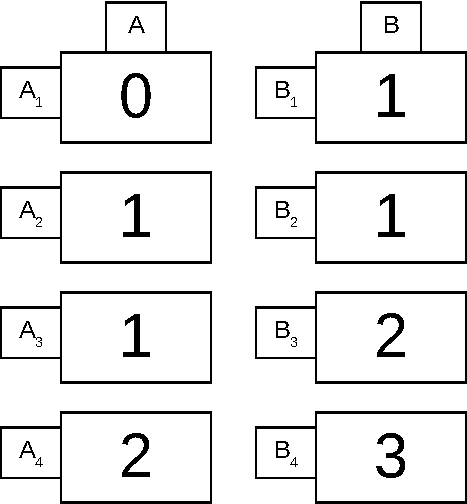
\includegraphics[width=\textwidth]{\zkevmdir/architecture/figures/fibonacci-sequence}
\end{figure}
\end{column}
%\hspace{-1.4cm}
\begin{column}{0.7\textwidth}
\begin{itemize}
\item The relations between the states of registries:
\begin{align*}
A_{i+1} &= B_i, \\
B_{i+1} &= A_i + B_i,
\end{align*}
for $i \in [4]$.
\item Are translated into relations (A.K.A identities) in the polynomial setting:
\begin{align*}
A(x\omega) &= \bigg\lvert_H  B(x), \\
B(x\omega) &= \bigg\lvert_H  A(x) + B(x).
\end{align*}
\end{itemize}
\end{column}
\end{columns}


%% iii
\begin{columns}
\begin{column}{0.3\textwidth}
\begin{figure}
	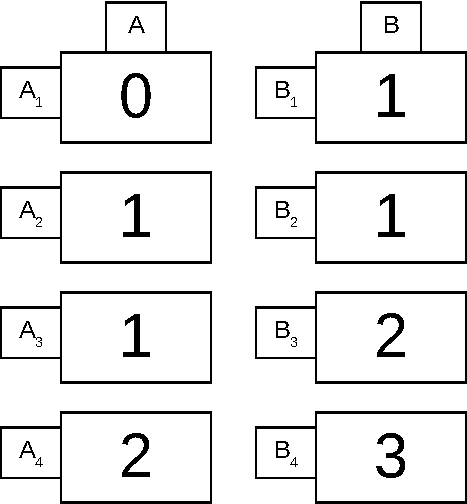
\includegraphics[width=\textwidth]{\zkevmdir/architecture/figures/fibonacci-sequence}
\end{figure}
\end{column}
%\hspace{-1.4cm}
\begin{column}{0.7\textwidth}

\begin{itemize}
\item So we have:

\vspace{-0.8cm}
\begin{align*}
A(x\omega) = \bigg\lvert_H  B(x), \quad
B(x\omega) = \bigg\lvert_H  A(x) + B(x).
\end{align*}
\item However, the previous identities do not correctly and uniquely describe our sequence because:
\begin{enumerate}
\item When we evaluate the identities in $\omega^4$:
\begin{align*}
A(\omega^5) = A(\omega) = 0 &\neq  3 = B(\omega^4), \\
B(\omega^5) = B(\omega) = 1 &\neq  5 = A(\omega^4) + B(\omega^4).
\end{align*}

The equations are not cyclic.
\item Other initial conditions also fulfill the identities, e.g:
$(2,3),(3,5),(5,8),(8,13)$.
\end{enumerate}
\end{itemize}
\end{column}
\end{columns}



%% iv
\begin{columns}
\begin{column}{0.4\textwidth}
\begin{figure}
	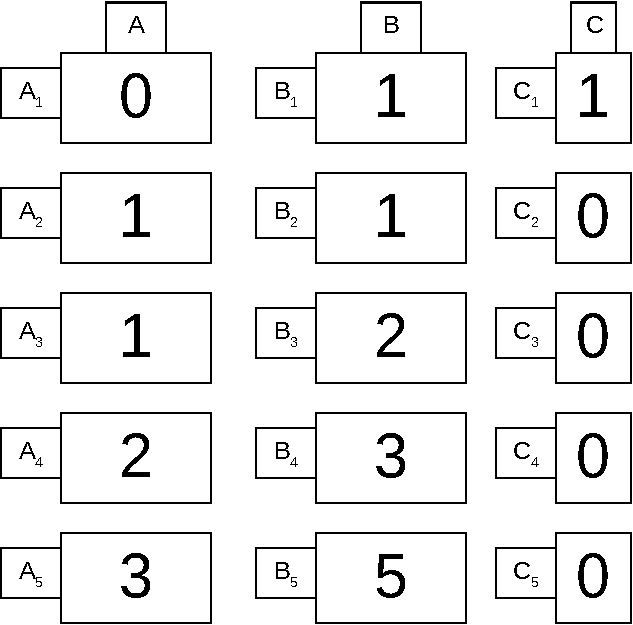
\includegraphics[width=\textwidth]{\zkevmdir/architecture/figures/fibonacci-sequence-aux}
\end{figure}
\end{column}
%\hspace{-1.4cm}
\begin{column}{0.6\textwidth}
\begin{itemize}
\item Let's add an auxiliary registry $C$ to solve these problems.
\item The corresponding polynomial is:
\begin{align*}
C(\omega^i) &= C_i \quad \Longrightarrow \quad C = [1, 0, 0, 0].
\end{align*}
\item With this auxiliary registry, we can now fix the polynomial identities as follows:
\begin{align*}
A(x\omega) &= \bigg\lvert_H  B(x)(1 - C(x\omega)), \\
B(x\omega) &= \bigg\lvert_H (A(x) + B(x))(1 - C(x\omega)) + C(x\omega).
\end{align*}
%\begin{align*}
%C(x)A(x) &= 0, \\
%C(x)(B(x) - 1) &= 0, \\
%A(x\omega) &=  B(x), \\
%B(x\omega) &=  A(x) + B(x).
%\end{align*}
\end{itemize}
\end{column}
\end{columns}


%% v
\begin{columns}
\begin{column}{0.4\textwidth}
\begin{figure}
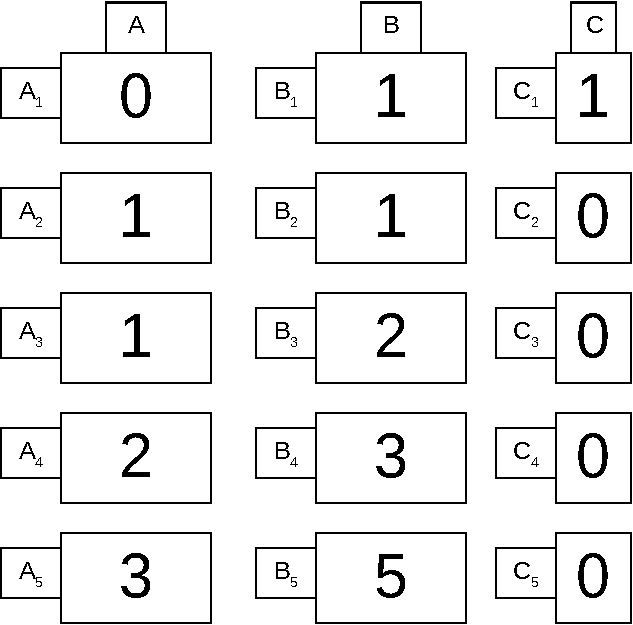
\includegraphics[width=\textwidth]{\zkevmdir/architecture/figures/fibonacci-sequence-aux}
\end{figure}
$C(x)$ is publicly known (A.K.A \textbf{pre-processed} or \textbf{constant}).
\end{column}

\begin{column}{0.6\textwidth}
\begin{itemize}
\item Note that now at $x = w^4$ the identities are satisfied:
\begin{align*}
A(x\omega) &= \bigg\lvert_H  B(x)(1 - C(x\omega)), \\
B(x\omega) &= \bigg\lvert_H (A(x) + B(x))(1 - C(x\omega)) + C(x\omega).\\
A(\omega^4 \omega) &= A(\omega^5) = A(\omega) = 0, \\
B(\omega^4 \omega) &= B(\omega^5) = B(\omega) = 1.
\end{align*}
\item We can also use other initial conditions $(A_0, B_0)$:
\begin{align*}
A(x\omega) &= \bigg\lvert_H  B(x)(1 - C(x\omega))+ A_0C(x\omega), \\
B(x\omega) &= \bigg\lvert_H  (A(x) + B(x))(1 - C(x\omega)) + B_0 C(x\omega).
\end{align*}
\end{itemize}
\end{column}
\end{columns}
\end{frame}





\begin{frame}[allowframebreaks]{Proving our State Machine (High Level)}
\begin{align*}
p_1(x)&= A(x\omega) - B(x)(1 - C(x\omega)) - A_0C(x\omega) = \bigg\lvert_H 0,\\
p_2(x) &= B(x\omega) - (A(x) + B(x))(1 - C(x\omega)) - B_0 C(x\omega) = \bigg\lvert_H 0.
\end{align*}

\begin{itemize}
\item We are going to convert these H-ranged identities into an $\FF$-ranged identities that 
is valid for any $x \in \FF$.
\item To do so, we are going to use the \textbf{zero polynomial} $Z_H(x)$.
\item $Z_H(x)$ is computed as the polynomial that is zero in $H$:
\[
(\omega,0), (\omega^2,0), (\omega^3,0), (\omega^4,0) \quad \Longrightarrow \quad Z_H(x) = (x-\omega)(x-\omega^2)(x-\omega^3)(x-\omega^4) = x^4-1.
\]

\item Notice that $p_1(x)$ and $p_2(x)$ have roots at $H$.
\item That means $Z_H(x) | p_1(x)$ and $Z_H(x) | p_2(x)$ 
because $(x-\omega)$, $(x-\omega^2)$, etc. are monomials of $p_1(x)$ and  $p_2(x)$.
\item Now we can compute $d_1(x) = p_1(x) / Z_H(x)$ and $d_2(x) = p_2(x) / Z_H(x)$.
\item The identities that need to be checked are $p_1(x) - d_1(x)Z_H(x) = 0$ and $p_2(x) - d_2(x)Z_H(x) = 0$ 
for any $x \in \FF$.
\end{itemize}

\begin{figure}
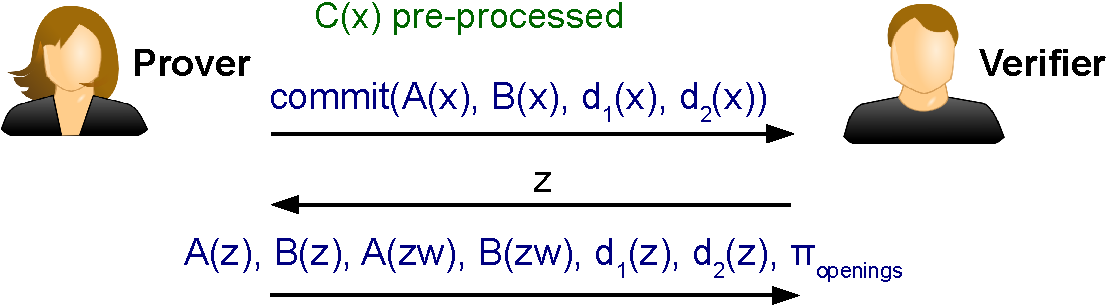
\includegraphics[width=0.8\columnwidth]{\zkevmdir/architecture/figures/proving_fibonacci}
\end{figure}
\end{frame}

% !TeX spellcheck = en_GB
% !TeX root = ../../build/zkEVM-architecture.tex

\section{$\mu$VM Architecture}

%TODO: Think this figure a little bit more to a better organization
\begin{frame}{$\mu$VM Architecture}
\begin{figure}
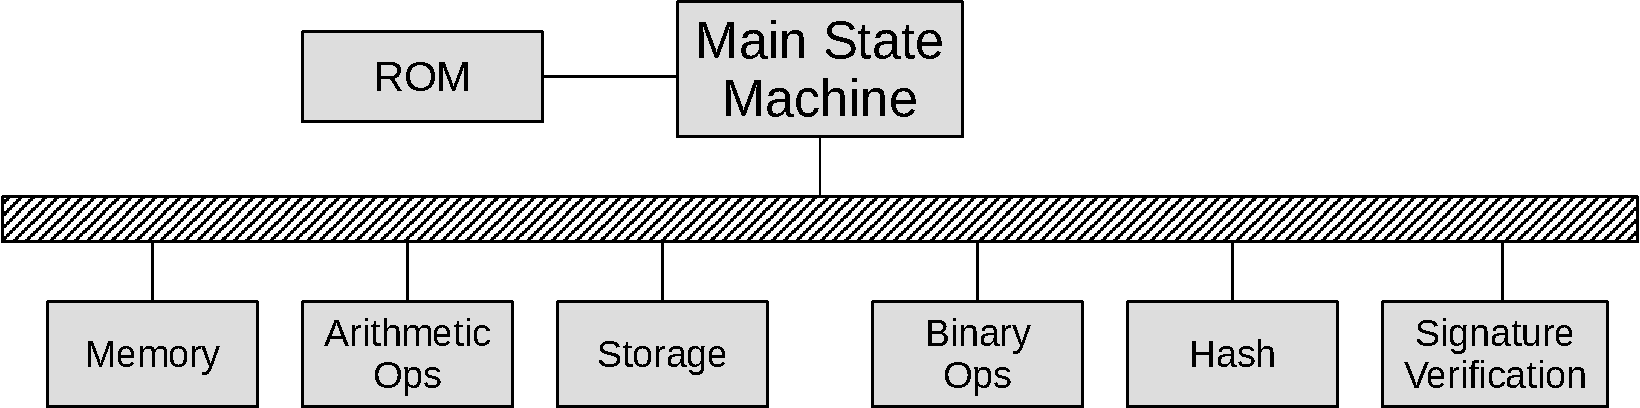
\includegraphics[width=\textwidth]{\zkevmdir/architecture/figures/microVM-architecture}
\end{figure}
All the relations between the different state machines are described as polynomial identities.
\end{frame}
% !TeX spellcheck = en_GB
% !TeX root = ../../build/zkEVM-architecture.tex

\section{Main State Machine}



\begin{frame}{Main State Machine of a Simplified Virtual Machine}
\begin{figure}
	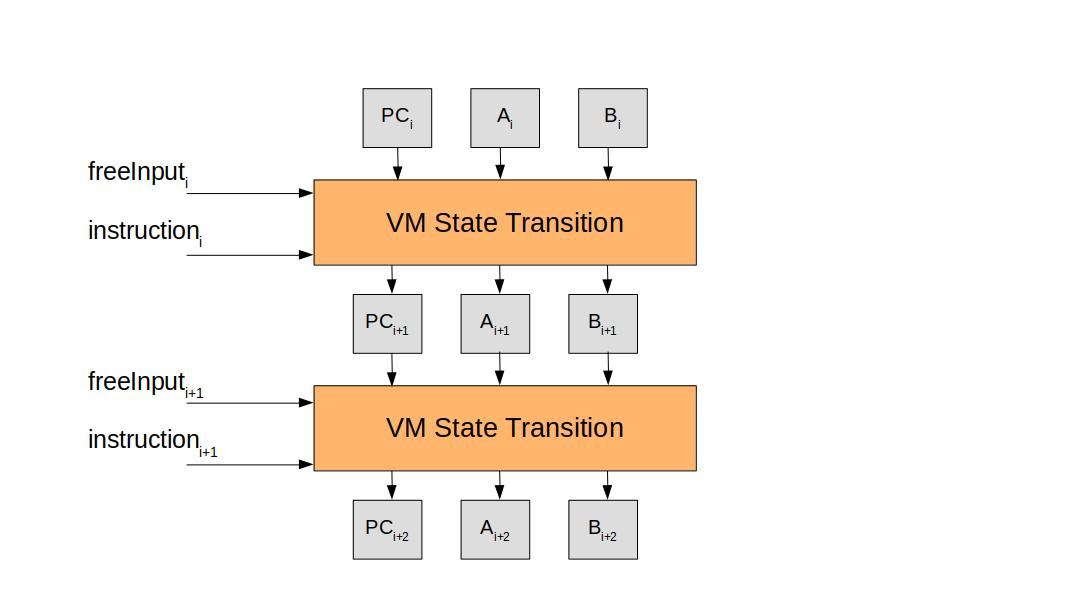
\includegraphics[width=0.65\textwidth]{main-state-machine-simplified-overview}
\end{figure}
\end{frame}
















\begin{frame}[allowframebreaks]{Example Program}
\begin{itemize}
\item Let's now work with a real program:
\[
\begin{array}{|c|l|c|}
\hline
\mathbf{Position} & \multicolumn{2}{|c|}{\mathbf{Instruction}} \\ \hline
0 & \mathbf{FREELOAD} & A \\ \hline
1 & \mathbf{MOV} & B, 3 \\ \hline
2 & \mathbf{JMP}~(if~B = 0) & 6 \\ \hline
3 & \mathbf{MUL} & A, A \\ \hline
4 & \mathbf{DEC} & B \\ \hline
5 & \mathbf{JMP} & 2 \\ \hline
6 & \mathbf{STOP} & \emptyset \\ \hline
\end{array}
\]

\item First, we encode each instruction in hexadecimal as follows:
\begin{columns}
\begin{column}{0.5\textwidth}
\begin{align*}
\mathbf{FREELOAD}~A &\to 0x00010000 \\
\mathbf{MOV}~B,n &\to 0x00020000 + n \\
\mathbf{JMP}~(if~B = 0)~n &\to 0x00040000 + n \\
\mathbf{JMP}~n &\to 0x00080000 + n \\
\mathbf{MUL}~A,A &\to 0x00100000 \\
\mathbf{DEC}~B &\to 0x00200000 \\
\mathbf{STOP} &\to 0x00400000 
\end{align*}
\end{column}
\begin{column}{0.5\textwidth}
\[
\begin{array}{|c|l|c|c|}
\hline
\mathbf{Position} & \multicolumn{2}{|c|}{\mathbf{Instruction}} & \mathbf{Inst.~Value}\\ \hline
0 & \mathbf{FREELOAD} & A & 0x00010000 \\ \hline
1 & \mathbf{MOV} & B, 3 & 0x00020003 \\ \hline
2 & \mathbf{JMP}~(if~B = 0) & 6 & 0x00040006 \\ \hline
3 & \mathbf{MUL} & A, A & 0x00100000 \\ \hline
4 & \mathbf{DEC} & B & 0x00200000 \\ \hline
5 & \mathbf{JMP} & 2 & 0x00080002 \\ \hline
6 & \mathbf{STOP} & \emptyset & 0x00400000 \\ \hline
\end{array}
\]
\end{column}
\end{columns}

\framebreak
\item With the support of this encoding, now we can compute the whole trace of the execution of this program:
\end{itemize}
\scriptsize
\[
\begin{array}{|c|l|c|c|c|c|c|c|}
\hline
\mathbf{Position} & \multicolumn{2}{|c|}{\mathbf{Instruction}} & \mathbf{Inst.~Value} & \mathbf{freeLoad} & \mathbf{PC} & \mathbf{A} & \mathbf{B} \\ \hline
0 & \mathbf{FREELOAD} & A & 0x00010000 & 10 & 0 & 0 & 0 \\ \hline
1 & \mathbf{MOV} & B, 3 & 0x00020003 & 0 & 1 & 10 & 0 \\ \hline
2 & \mathbf{JMP}~(if~B = 0) & 6 & 0x00040006 & 0 & 2 & 10 & 3 \\ \hline
3 & \mathbf{MUL} & A, A & 0x00100000 & 0 & 3 & 10 & 3 \\ \hline
4 & \mathbf{DEC} & B & 0x00200000 & 0 & 4 & 100 & 3 \\ \hline
5 & \mathbf{JMP} & 2 & 0x00080002 & 0 & 5 & 100 & 2 \\ \hline
6 & \mathbf{JMP}~(if~B = 0) & 6 & 0x00040006 & 0 & 2 & 100 & 2 \\ \hline
7 & \mathbf{MUL} & A, A & 0x00100000 & 0 & 3 & 100 & 2 \\ \hline
8 & \mathbf{DEC} & B & 0x00200000 & 0 & 4 & 1000 & 2 \\ \hline
9 & \mathbf{JMP} & 2 & 0x00080002 & 0 & 5 & 1000 & 1 \\ \hline
10 & \mathbf{JMP}~(if~B = 0) & 6 & 0x00040006 & 0 & 2 & 1000 & 1 \\ \hline
11 & \mathbf{MUL} & A, A & 0x00100000 & 0 & 3 & 1000 & 1 \\ \hline
12 & \mathbf{DEC} & B & 0x00200000 & 0 & 4 & 10000 & 1 \\ \hline
13 & \mathbf{JMP} & 2 & 0x00080002 & 0 & 5 & 10000 & 0 \\ \hline
14 & \mathbf{JMP}~(if~B = 0) & 6 & 0x00040006 & 0 & 2 & 10000 & 0 \\ \hline
15 & \mathbf{STOP} & \emptyset & 0x00400000 & 0 & 6 & 10000 & 0 \\ \hline
\end{array}
\]
\end{frame}





\begin{frame}[allowframebreaks]{Checking the Correct Program Execution}
\begin{itemize}
\item The question that arises now is:
\begin{center}
\textbf{How do we actually verify that we are executing the correct program?}
\end{center}

\item The solution seems obvious: Check that every row of the trace of the execution coincides with some row of the program.

\item Then, the question becomes to:
\begin{center}
\textbf{How do we actually verify that we are executing the correct program \\ in an efficient manner?}
\end{center}

\item We can do it with Plookup!

\framebreak

\item On the one side:
\[
\begin{array}{|c|l|c|c|c|}
\hline
\mathbf{Position} & \multicolumn{2}{|c|}{\mathbf{Instruction}} & \mathbf{Inst.~Value} & \mathbf{Rom} = \mathbf{inst} + 2^{32} \cdot \mathbf{position} \\ \hline
0 & \mathbf{FREELOAD} & A & 0x00010000 & 0x0.00010000 \\ \hline
1 & \mathbf{MOV} & B, 3 & 0x00020003 & 0x1.00020003 \\ \hline
2 & \mathbf{JMP}~(if~B = 0) & 6 & 0x00040006 & 0x2.00040006 \\ \hline
3 & \mathbf{MUL} & A, A & 0x00100000 & 0x3.00100000 \\ \hline
4 & \mathbf{DEC} & B & 0x00200000 & 0x4.00200000 \\ \hline
5 & \mathbf{JMP} & 2 & 0x00080002 & 0x5.00080002 \\ \hline
6 & \mathbf{STOP} & \emptyset & 0x00400000 & 0x6.00400000 \\ \hline
\end{array}
\]

\item On the other side:
\scriptsize
\[
\begin{array}{|c|l|c|c|c|c|c|c|c|}
\hline
\mathbf{Position} & \multicolumn{2}{|c|}{\mathbf{Instruction}} & \mathbf{Inst.~Value} & \mathbf{freeLoad} & \mathbf{PC} & \mathbf{A} & \mathbf{B} &  \mathbf{instTrace} = \mathbf{inst} + 2^{32} \cdot \mathbf{PC} \\ \hline
0 & \mathbf{FREELOAD} & A & 0x00010000 & 10 & 0 & 0 & 0 & 0x0.00010000 \\ \hline
1 & \mathbf{MOV} & B, 3 & 0x00020003 & 0 & 1 & 10 & 0 & 0x1.00020003 \\ \hline
2 & \mathbf{JMP}~(if~B = 0) & 6 & 0x00040006 & 0 & 2 & 10 & 3 & 0x2.00040006 \\ \hline
3 & \mathbf{MUL} & A, A & 0x00100000 & 0 & 3 & 10 & 3 & 0x3.00100000 \\ \hline
4 & \mathbf{DEC} & B & 0x00200000 & 0 & 4 & 100 & 3 & 0x4.00200000 \\ \hline
5 & \mathbf{JMP} & 2 & 0x00080002 & 0 & 5 & 100 & 2 & 0x5.00080002 \\ \hline
6 & \mathbf{JMP}~(if~B = 0) & 6 & 0x00040006 & 0 & 2 & 100 & 2 & 0x2.00040006 \\ \hline
7 & \mathbf{MUL} & A, A & 0x00100000 & 0 & 3 & 100 & 2 & 0x3.00100000 \\ \hline
8 & \mathbf{DEC} & B & 0x00200000 & 0 & 4 & 1000 & 2 & 0x4.00200000 \\ \hline
9 & \mathbf{JMP} & 2 & 0x00080002 & 0 & 5 & 1000 & 1 & 0x5.00080002 \\ \hline
10 & \mathbf{JMP}~(if~B = 0) & 6 & 0x00040006 & 0 & 2 & 1000 & 1 & 0x2.00040006 \\ \hline
11 & \mathbf{MUL} & A, A & 0x00100000 & 0 & 3 & 1000 & 1 & 0x3.00100000 \\ \hline
12 & \mathbf{DEC} & B & 0x00200000 & 0 & 4 & 10000 & 1 & 0x4.00200000 \\ \hline
13 & \mathbf{JMP} & 2 & 0x00080002 & 0 & 5 & 10000 & 0 & 0x5.00080002 \\ \hline
14 & \mathbf{JMP}~(if~B = 0) & 6 & 0x00040006 & 0 & 2 & 10000 & 0 & 0x2.00040006 \\ \hline
15 & \mathbf{STOP} & \emptyset & 0x00400000 & 0 & 6 & 10000 & 0 & 0x6.00400000 \\ \hline
\end{array}
\]

\normalsize
\item So, to check that the correct program is being executed, we simply have to use Plookup to determine if:
\[
\mathbf{instTrace} \subset \mathbf{Rom}
\]

\item In simple words, the trace being executed is an execution of the actual program if the instruction trace is contained in the ROM of the program.
\end{itemize}
\end{frame}









\subsection{Storage}
\begin{frame}{Main State Machine of a Virtual Machine}
\begin{figure}
	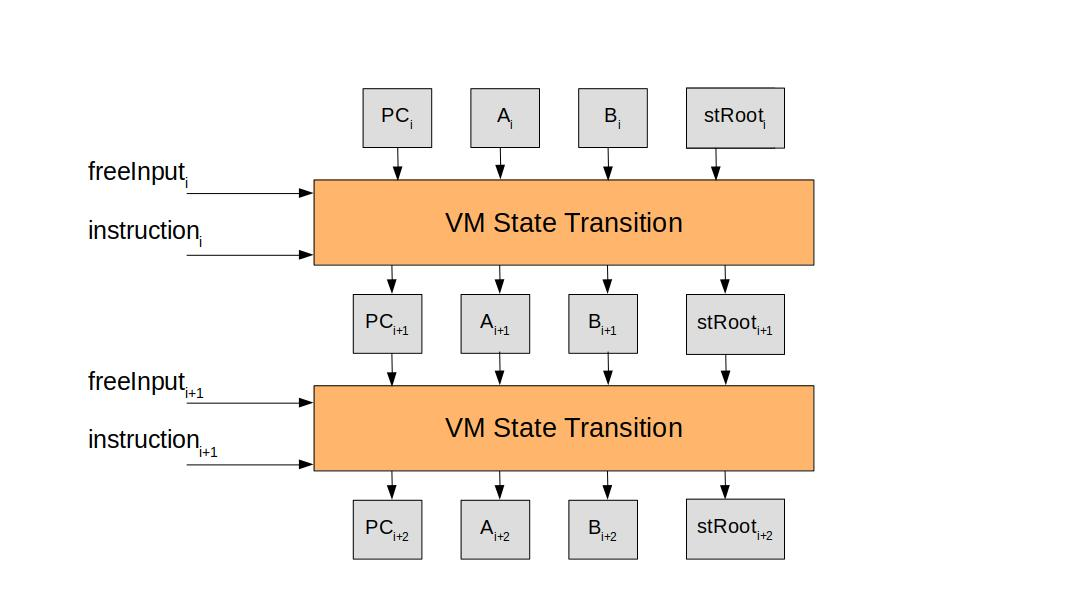
\includegraphics[width=0.65\textwidth]{main-state-machine-overview}
\end{figure}
\end{frame}







\begin{frame}{Main State Machine of a Virtual Machine}
\scriptsize
\[
\begin{array}{|c|l|c|c|c|c|c|c|c|c|c|c|}
\hline
\mathbf{Position} & \multicolumn{2}{|c|}{\mathbf{Instruction}} & \mathbf{freeLoad} & \mathbf{stRoot} & \mathbf{A} & \mathbf{B} & \mathbf{oldStRoot} & \mathbf{newStRoot} & \mathbf{Key} & \mathbf{Value} \\ \hline
0 &  &  &  & \mathsf{st1} &  &  & 0 & 0 & 0 & 0 \\ \hline
1 &  &  &  & \mathsf{st1} &  &  & 0 & 0 & 0 & 0 \\ \hline
2 &  &  &  & \mathsf{st1} &  &  & 0 & 0 & 0 & 0 \\ \hline
3 & \mathbf{SSTORE} & [A], B & \mathsf{st2} & \mathsf{st1} & 0x4C76 & 1232 & \mathsf{st1} & \mathsf{st2} & 0x4C76 & 1232 \\ \hline
4 &  &  &  & \mathsf{st2} & 0x4C76 & 1232 & 0 & 0 & 0 & 0 \\ \hline
5 &  &  &  & \mathsf{st2} &  &  & 0 & 0 & 0 & 0 \\ \hline
6 &  &  &  & \mathsf{st2} &  &  & 0 & 0 & 0 & 0 \\ \hline
7 & \mathbf{SSTORE} & [A], B & \mathsf{st3} & \mathsf{st2} & 0x8E12 & 7765 & \mathsf{st2} & \mathsf{st3} & 0x8E12 & 7765 \\ \hline
8 &  &  &  & \mathsf{st3} & 0x8E12 & 7765 & 0 & 0 & 0 & 0 \\ \hline
9 &  &  &  & \mathsf{st3} &  &  & 0 & 0 & 0 & 0 \\ \hline
10 & \mathbf{SSTORE} & [A], B & \mathsf{st4} & \mathsf{st3} & 0xAA23 & 9812 & \mathsf{st3} & \mathsf{st4} & 0xAA23 & 9812 \\ \hline
11 &  &  &  & \mathsf{st4} & 0xAA23 & 9812 & 0 & 0 & 0 & 0 \\ \hline
12 &  &  &  & \mathsf{st4} &  &  & 0 & 0 & 0 & 0 \\ \hline
13 &  &  &  & \mathsf{st4} &  &  & 0 & 0 & 0 & 0 \\ \hline
14 & \mathbf{SSTORE} & [A], B & \mathsf{st5} & \mathsf{st4} & 0x2213 & 8610 & \mathsf{st4} & \mathsf{st5} & 0x2213 & 8610 \\ \hline
15 &  &  &  & \mathsf{st5} & 0x2213 & 8610 & 0 & 0 & 0 & 0 \\ \hline
\end{array}
\]
\end{frame}







\subsection{Memory}


\begin{frame}{Memory in the Main State Machine}
\scriptsize
\[
\begin{array}{|c|l|c|c|c|c|c|c|c|c|c|}
\hline
\mathbf{Position} & \multicolumn{2}{|c|}{\mathbf{Instruction}} & \mathbf{freeLoad}  & \mathbf{A} & \mathbf{B} & \mathbf{mRead} & \mathbf{mWrite} & \mathbf{Address} & \mathbf{Value} \\ \hline
0 &  &  &  &  &  & 0 & 0 & 0 & 0 \\ \hline
1 &  &  &  &  &  & 0 & 0 & 0 & 0 \\ \hline
2 &  &  &  &  &  & 0 & 0 & 0 & 0 \\ \hline
3 & \mathbf{MWRITE} & [A], B &  & 0x4C76 & 1232 & 0 & 1 & 0x4C76 & 1232 \\ \hline
4 &  &  &  & 0x4C76 & 1232 & 0 & 0 & 0 & 0 \\ \hline
5 & \mathbf{MREAD} & B, [A] & 1232 & 0x4C76 & 1232 & 1 & 0 & 0x4C76 & 1232 \\ \hline
6 &  &  &  & 0x4C76 & 1232 & 0 & 0 & 0 & 0 \\ \hline
7 & \mathbf{MWRITE} & [A], B &  & 0x8E12 & 7765 & 0 & 1 & 0x8E12 & 7765 \\ \hline
8 &  &  &  & 0x8E12 & 7765 & 0 & 0 & 0 & 0 \\ \hline
9 &  &  &  &  &  & 0 & 0 & 0 & 0 \\ \hline
10 & \mathbf{MWRITE} & [A], B &  & 0x2213 & 8610 & 0 & 1 & 0x2213 & 8610 \\ \hline
11 &  &  &  & 0x2213 & 8610 & 0 & 0 & 0 & 0 \\ \hline
12 &  &  &  &  &  & 0 & 0 & 0 & 0 \\ \hline
13 &  &  &  &  &  & 0 & 0 & 0 & 0 \\ \hline
14 & \mathbf{MREAD} & B, [A] & 7765 & 0x8E12 & 7765 & 1 & 0 & 0x8E12 & 7765 \\ \hline
15 &  &  &  & 0x8E12 & 7765 & 0 & 0 & 0 & 0 \\ \hline
\end{array}
\]
\end{frame}







\begin{frame}{Memory State Machine}
\scriptsize
\[
\begin{array}{|c|l|c|c|c|c|c|c|c|}
\hline
\multicolumn{5}{|c|}{\textbf{Free Inputs}} & \multicolumn{2}{|c|}{\textbf{Intermediary State}} & \mathbf{Results} \\ \hline
\mathbf{Position} & \textbf{mRead} & \textbf{mWrite} & \mathbf{Address}  & \mathbf{ValueIn} & \mathbf{stOld} & \mathbf{stNew} & \mathbf{Value} \\ \hline
%0 & 0 & 0 & 0 & 0 & 0 & 0 & 0 \\ \hline
3 & 0 & 1 & 0x4C76 & 1232 & 0 & 1232 & 1232 \\ \hline
5 & 1 & 0 & 0x4C76 &  & 1232 & 1232 & 1232 \\ \hline
7 & 0 & 1 & 0x8E12 & 7765 & 1232 & 7765 & 7765 \\ \hline
14 & 1 & 0 & 0x8E12 &  & 7765 & 7765 & 7765 \\ \hline
10 & 0 & 1 & 0x2213 & 8610 & 7765 & 8610 & 8610 \\ \hline
\end{array}
\]
\small
\begin{itemize}
\item Using Plookup, prove that the polynomial:
\[
main.position(x) + v \cdot main.mRead(x) + v^2 \cdot main.mWrite(x) + v^3 \cdot main.Address(x) + v^4 \cdot main.Value(x),
\]
is included in the polynomial:
\[
mem.position(x) + v \cdot mem.mRead(x) + v^2 \cdot mem.mWrite(x) + v^3 \cdot mem.Address(x) + v^4 \cdot mem.Value(x).
\]
\end{itemize}
\end{frame}







\subsection{Binary Operations}

\begin{frame}{Checking Binary Operations: XOR}
\begin{columns}
\footnotesize
\begin{column}{0.5\textwidth}
\begin{center}
\underline{\textbf{Operation}} \\[0.2cm]
$f(x) \xor g(x) = h(x)$.
\end{center}
\begin{enumerate}
\item Check byte decomposition:
\begin{align*}
f(x) &= f_0(x) + 2^8 f_1(x) + 2^{16} f_2(x) + \dots \\
g(x) &= g_0(x) + 2^8 g_1(x) + 2^{16} g_2(x) + \dots \\
h(x) &= h_0(x) + 2^8 h_1(x) + 2^{16} h_2(x) + \dots
\end{align*}

\item Check byte form elementwise:
\[
\begin{array}{ccc}
f_0(x) \subset \mathsf{byte(x)} & g_0(x) \subset \mathsf{byte(x)} & h_0(x) \subset \mathsf{byte(x)} \\
f_1(x) \subset \mathsf{byte(x)} & g_1(x) \subset \mathsf{byte(x)} & h_1(x) \subset \mathsf{byte(x)} \\
f_2(x) \subset \mathsf{byte(x)} & g_2(x) \subset \mathsf{byte(x)} & h_2(x) \subset \mathsf{byte(x)} \\
\vdots & \vdots & \vdots
\end{array}
\]
\end{enumerate}
\end{column}
\begin{column}{0.5\textwidth}
\begin{enumerate}
\item[3.] Check $\XOR$ operation:
\[
\begin{array}{c}
f_0(x) + 2^8 g_0(x) + 2^{16} h_0(x) \subset \XOR(x) \\
f_1(x) + 2^8 g_1(x) + 2^{16} h_1(x) \subset \XOR(x) \\
f_2(x) + 2^8 g_2(x) + 2^{16} h_2(x) \subset \XOR(x) \\
\vdots
\end{array}
\]
\end{enumerate}
\[
\begin{array}{|c|c|}
\hline
\mathbf{x} & \mathbf{byte} \\ \hline
\omega^0 & 0x00 \\ \hline
\omega^1 & 0x01 \\ \hline
\vdots & \vdots \\ \hline
\omega^{123} & 0x7B \\ \hline
\vdots & \vdots \\ \hline
\omega^{255} & 0xFF \\ \hline
\end{array}
\hspace{1cm}
\begin{array}{|c|c|}
\hline
\mathbf{x} & \XOR \\ \hline
\omega^0 & 0x000000 \\ \hline
\omega^1 & 0x010001 \\ \hline
\vdots & \vdots \\ \hline
\omega^{5028} & 0xB713A4 \\ \hline
\vdots & \vdots \\ \hline
\omega^{65535} & 0x00FFFF \\ \hline
\end{array}
\]
\end{column}
\end{columns}
\end{frame}










\subsection{Arithmetic Operations}

\begin{frame}{Checking Arithmetic Operations: Multiplication}
\scriptsize
\begin{columns}
\begin{column}{0.5\textwidth}
\begin{figure}
	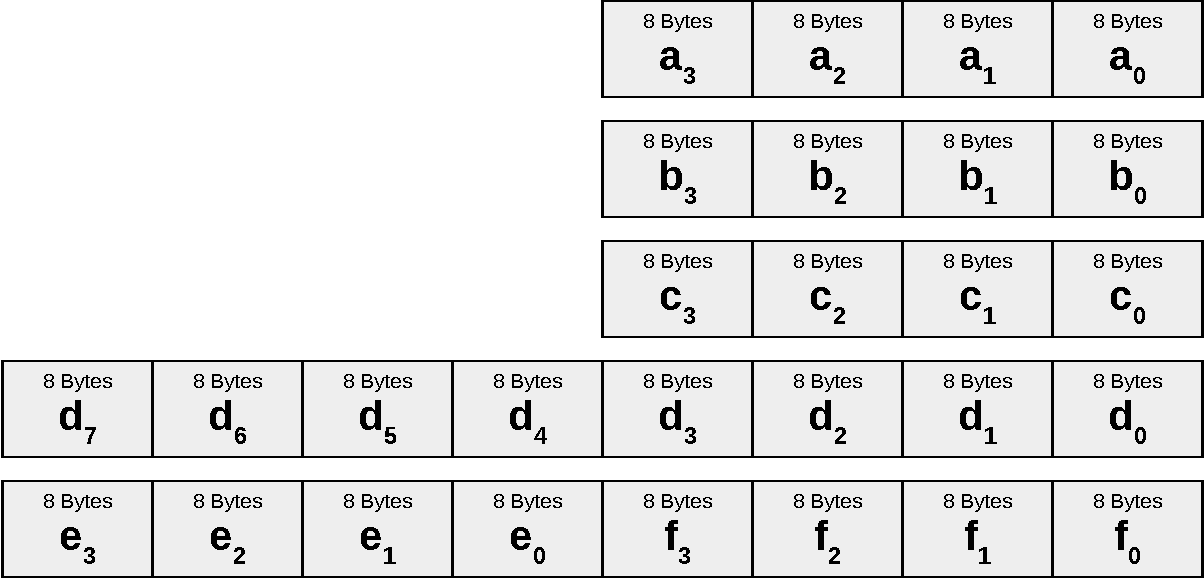
\includegraphics[width=0.8\textwidth]{multiplication}
\end{figure}
\end{column}
\begin{column}{0.5\textwidth}
\begin{align*}
A = &~a_2 \cdot 256^{22} + a_1 \cdot 256^{11} + a_0, \\
B = &~b_2 \cdot 256^{22} + b_1 \cdot 256^{11} + b_0, \\
C = &~c_2 \cdot 256^{22} + c_1 \cdot 256^{11} + c_0, \\
D = &~d_5 \cdot 256^{55} + d_4 \cdot 256^{44} + d_3 \cdot 256^{33} \\
&+ d_2 \cdot 256^{22} + d_1 \cdot 256^{11} + d_0, \\
E = &~e_2 \cdot 256^{22} + e_1 \cdot 256^{11} + e_0, \\
F = &~f_2 \cdot 256^{22} + f_1 \cdot 256^{11} + f_0,
\end{align*}
\end{column}
\end{columns}
\begin{columns}
\begin{column}{0.33\textwidth}
\[
A \cdot B + C = D = E \cdot 2^{256} + F
\]
\end{column}
\begin{column}{0.33\textwidth}
\begin{align*}
&d_0 = f_0, \\
&d_1 = f_1, \\
&d_2 = f_2 + \mathsf{carry_1} \cdot 256^{10}, \\
&d_3 \cdot 256 + \mathsf{carry_1} = e_0 + \mathsf{carry_2} \cdot 256^{11}, \\
&d_4 \cdot 256 + \mathsf{carry_2} = e_1 + \mathsf{carry_3} \cdot 256^{11}, \\
&d_5 \cdot 256 + \mathsf{carry_3} = e_1.
\end{align*}
\end{column}
\begin{column}{0.33\textwidth}
\[
\mathsf{carry_1}, \mathsf{carry_2}, \mathsf{carry_3} \subset \mathsf{byte}.
\]
\end{column}
\end{columns}
\end{frame}









\begin{frame}{Multiplying}
\scriptsize
\[
\begin{array}{|c|c|c|c|c|c|c|c|c|c|c|c|c|c|c|c|c|c|c|}
\hline
\mathbf{Step} & \mathbf{mA} & \mathbf{mB} & \mathbf{acc_5} & \mathbf{acc_4}  & \mathbf{acc_3} & \mathbf{acc_2} & \mathbf{acc_1} & \mathbf{acc_0} \\ \hline
0 & a_0 & b_0 & d_5 & d_4 & d_3 & d_2 & d_1 & d_0 \\ \hline
1 & a_0 & b_1 & d_0 & d_5 & d_4 & d_3 & d_2 & d_1 \\ \hline
2 & a_1 & b_0 & d_0 & d_5 & d_4 & d_3 & d_2 & d_1 \\ \hline
3 & a_0 & b_2 & d_1 & d_0 & d_5 & d_4 & d_3 & d_2 \\ \hline
4 & a_1 & b_1 & d_1 & d_0 & d_5 & d_4 & d_3 & d_2 \\ \hline
5 & a_2 & b_0 & d_1 & d_0 & d_5 & d_4 & d_3 & d_2 \\ \hline
6 & a_1 & b_2 & d_2 & d_1 & d_0 & d_5 & d_4 & d_3 \\ \hline
7 & a_2 & b_1 & d_2 & d_1 & d_0 & d_5 & d_4 & d_3 \\ \hline
8 & a_2 & b_2 & d_3 & d_2 & d_1 & d_0 & d_5 & d_4 \\ \hline
\end{array}
\]
\[
\hspace{2.5cm}
\begin{array}{|c|c|c|c|c|c|c|c|c|c|c|c|c|c|c|c|c|c|c|}
\hline
\mathbf{q_{shift}} & \mathbf{q_{same}} & \mathbf{q_{set}} & \mathbf{q_{result}} & \mathbf{q_{a_0}} & \mathbf{q_{a_1}} & \mathbf{q_{a_2}} & \mathbf{q_{b_0}} & \mathbf{q_{b_1}} & \mathbf{q_{b_2}} \\ \hline
0 & 0 & 1 & 0 & 1 & 0 & 0 & 1 & 0 & 0\\ \hline
1 & 0 & 0 & 0 & 1 & 0 & 0 & 0 & 1 & 0\\ \hline
0 & 1 & 0 & 0 & 0 & 1 & 0 & 1 & 0 & 0\\ \hline
1 & 0 & 0 & 0 & 1 & 0 & 0 & 0 & 0 & 1\\ \hline
0 & 1 & 0 & 0 & 0 & 1 & 0 & 0 & 1 & 0\\ \hline
0 & 1 & 0 & 0 & 0 & 0 & 1 & 1 & 0 & 0\\ \hline
1 & 0 & 0 & 0 & 0 & 1 & 0 & 0 & 0 & 1\\ \hline
0 & 1 & 0 & 0 & 0 & 0 & 1 & 0 & 1 & 0\\ \hline
1 & 0 & 0 & 1 & 0 & 0 & 1 & 0 & 0 & 1\\ \hline
\end{array}
\]
\end{frame}

	
\end{document}